% Für Bindekorrektur als optionales Argument "BCORfaktormitmaßeinheit", dann
% sieht auch Option "twoside" vernünftig aus
% Näheres zu "scrartcl" bzw. "scrreprt" und "scrbook" siehe KOMA-Skript Doku
\documentclass[12pt,a4paper,titlepage,headinclude,bibtotoc]{scrartcl}


%---- Allgemeine Layout Einstellungen ------------------------------------------

% Für Kopf und Fußzeilen, siehe auch KOMA-Skript Doku
\usepackage[komastyle]{scrpage2}
\pagestyle{scrheadings}
\setheadsepline{0.5pt}[\color{black}]
\automark[section]{chapter}


%Einstellungen für Figuren- und Tabellenbeschriftungen
\setkomafont{captionlabel}{\sffamily\bfseries}
\setcapindent{0em}


%---- Weitere Pakete -----------------------------------------------------------
% Die Pakete sind alle in der TeX Live Distribution enthalten. Wichtige Adressen
% www.ctan.org, www.dante.de

% Sprachunterstützung
\usepackage[ngerman]{babel}

% Benutzung von Umlauten direkt im Text
% entweder "latin1" oder "utf8"
\usepackage[utf8]{inputenc}

% Pakete mit Mathesymbolen und zur Beseitigung von Schwächen der Mathe-Umgebung
\usepackage{latexsym,exscale,stmaryrd,amssymb,amsmath}

% Weitere Symbole
\usepackage[nointegrals]{wasysym}
\usepackage{eurosym}

% Anderes Literaturverzeichnisformat
%\usepackage[square,sort&compress]{natbib}

% Für Farbe
\usepackage{color}

% Zur Graphikausgabe
%Beipiel: \includegraphics[width=\textwidth]{grafik.png}
\usepackage{graphicx}

% Text umfließt Graphiken und Tabellen
% Beispiel:
% \begin{wrapfigure}[Zeilenanzahl]{"l" oder "r"}{breite}
%   \centering
%   \includegraphics[width=...]{grafik}
%   \caption{Beschriftung} 
%   \label{fig:grafik}
% \end{wrapfigure}
\usepackage{wrapfig}

% Mehrere Abbildungen nebeneinander
% Beispiel:
% \begin{figure}[htb]
%   \centering
%   \subfigure[Beschriftung 1\label{fig:label1}]
%   {\includegraphics[width=0.49\textwidth]{grafik1}}
%   \hfill
%   \subfigure[Beschriftung 2\label{fig:label2}]
%   {\includegraphics[width=0.49\textwidth]{grafik2}}
%   \caption{Beschriftung allgemein}
%   \label{fig:label-gesamt}
% \end{figure}
\usepackage{subfigure}

% Caption neben Abbildung
% Beispiel:
% \sidecaptionvpos{figure}{"c" oder "t" oder "b"}
% \begin{SCfigure}[rel. Breite (normalerweise = 1)][hbt]
%   \centering
%   \includegraphics[width=0.5\textwidth]{grafik.png}
%   \caption{Beschreibung}
%   \label{fig:}
% \end{SCfigure}
\usepackage{sidecap}

% Befehl für "Entspricht"-Zeichen
\newcommand{\corresponds}{\ensuremath{\mathrel{\widehat{=}}}}

%Für chemische Formeln (von www.dante.de)
%% Anpassung an LaTeX(2e) von Bernd Raichle
\makeatletter
\DeclareRobustCommand{\chemical}[1]{%
  {\(\m@th
   \edef\resetfontdimens{\noexpand\)%
       \fontdimen16\textfont2=\the\fontdimen16\textfont2
       \fontdimen17\textfont2=\the\fontdimen17\textfont2\relax}%
   \fontdimen16\textfont2=2.7pt \fontdimen17\textfont2=2.7pt
   \mathrm{#1}%
   \resetfontdimens}}
\makeatother


%erzwinge Fussnote auf selber Seite
\interfootnotelinepenalty=1000
\usepackage{supertabular}

%c++ Code einbinden
\usepackage{listings}
\lstset{numbers=left, numberstyle=\tiny, numbersep=5pt}

%Honneker Boxen
\usepackage{fancybox}

%Zitate
%\usepackage[round]{natbib}
\usepackage{cite}

%keine Einrückung nach leerzeile
\parindent0pt

%Literaturverzeichnis
\usepackage{babelbib}
\selectbiblanguage{ngerman}

%SI-Einheiten
\usepackage{siunitx}

\begin{document}

\begin{titlepage}
\centering
\textsc{\Large Anfängerpraktikum der Fakultät für
  Physik,\\[1.5ex] Universität Göttingen}

\vspace*{4.2cm}

\rule{\textwidth}{1pt}\\[0.5cm]
{\huge \bfseries
  Versuch Spezifische Wärme der Luft\\[1.5ex]
  Versuchsprotokoll}\\[0.5cm]
\rule{\textwidth}{1pt}

\vspace*{3cm}

\begin{Large}
\begin{tabular}{ll}
Praktikant: & Kevin Lüdemann  \\
%	& Skrollan Detzler\\
%	& Felix Kurtz\\
	& Michalel Lohmann\\
E-Mail: & kevin.luedemann@stud.uni-goettingen.de, \\
%       & skrollan.detzler@stud.uni-goettingen.de\\
	& m.lohmann@stud.uni-goettingen.de\\
%	& felix.kurtz@stud.uni-goettingen.de\\
Betreuer: & Martin Ochmann\\
Versuchsdatum: & 2.6.2014\\
\end{tabular}
\end{Large}

\vspace*{0.8cm}

\begin{Large}
\fbox{
  \begin{minipage}[t][2.5cm][t]{6cm} 
    Testat:
  \end{minipage}
}
\end{Large}

\end{titlepage}

\tableofcontents

\newpage

\section{Einleitung}
\label{sec:einleitung}



\section{Theorie}
\label{sec:theorie}



\section{Durchführung}
\label{sec:durchfuehrung}
\subsection{Gasthermometer}

\section{Auswertung}
\label{sec:auswertung}

\subsection{Gasthermometer}
Die Graphik \ref{fig:gas1} 
\subsubsection{Erwärmung des Gases}
\label{sec:gas1}
Da die Werte vom Druckmessgerät in kPa/2 ausgegeben werden, müssen alle Werte zum Druck aus dieser Messung mit Faktor zwei multipliziert und dazu der Normaldruck von 1013 hPa addiert werden.
\begin{figure}[!h]
\centering
% GNUPLOT: LaTeX picture with Postscript
\begingroup
  \makeatletter
  \providecommand\color[2][]{%
    \GenericError{(gnuplot) \space\space\space\@spaces}{%
      Package color not loaded in conjunction with
      terminal option `colourtext'%
    }{See the gnuplot documentation for explanation.%
    }{Either use 'blacktext' in gnuplot or load the package
      color.sty in LaTeX.}%
    \renewcommand\color[2][]{}%
  }%
  \providecommand\includegraphics[2][]{%
    \GenericError{(gnuplot) \space\space\space\@spaces}{%
      Package graphicx or graphics not loaded%
    }{See the gnuplot documentation for explanation.%
    }{The gnuplot epslatex terminal needs graphicx.sty or graphics.sty.}%
    \renewcommand\includegraphics[2][]{}%
  }%
  \providecommand\rotatebox[2]{#2}%
  \@ifundefined{ifGPcolor}{%
    \newif\ifGPcolor
    \GPcolortrue
  }{}%
  \@ifundefined{ifGPblacktext}{%
    \newif\ifGPblacktext
    \GPblacktexttrue
  }{}%
  % define a \g@addto@macro without @ in the name:
  \let\gplgaddtomacro\g@addto@macro
  % define empty templates for all commands taking text:
  \gdef\gplbacktext{}%
  \gdef\gplfronttext{}%
  \makeatother
  \ifGPblacktext
    % no textcolor at all
    \def\colorrgb#1{}%
    \def\colorgray#1{}%
  \else
    % gray or color?
    \ifGPcolor
      \def\colorrgb#1{\color[rgb]{#1}}%
      \def\colorgray#1{\color[gray]{#1}}%
      \expandafter\def\csname LTw\endcsname{\color{white}}%
      \expandafter\def\csname LTb\endcsname{\color{black}}%
      \expandafter\def\csname LTa\endcsname{\color{black}}%
      \expandafter\def\csname LT0\endcsname{\color[rgb]{1,0,0}}%
      \expandafter\def\csname LT1\endcsname{\color[rgb]{0,1,0}}%
      \expandafter\def\csname LT2\endcsname{\color[rgb]{0,0,1}}%
      \expandafter\def\csname LT3\endcsname{\color[rgb]{1,0,1}}%
      \expandafter\def\csname LT4\endcsname{\color[rgb]{0,1,1}}%
      \expandafter\def\csname LT5\endcsname{\color[rgb]{1,1,0}}%
      \expandafter\def\csname LT6\endcsname{\color[rgb]{0,0,0}}%
      \expandafter\def\csname LT7\endcsname{\color[rgb]{1,0.3,0}}%
      \expandafter\def\csname LT8\endcsname{\color[rgb]{0.5,0.5,0.5}}%
    \else
      % gray
      \def\colorrgb#1{\color{black}}%
      \def\colorgray#1{\color[gray]{#1}}%
      \expandafter\def\csname LTw\endcsname{\color{white}}%
      \expandafter\def\csname LTb\endcsname{\color{black}}%
      \expandafter\def\csname LTa\endcsname{\color{black}}%
      \expandafter\def\csname LT0\endcsname{\color{black}}%
      \expandafter\def\csname LT1\endcsname{\color{black}}%
      \expandafter\def\csname LT2\endcsname{\color{black}}%
      \expandafter\def\csname LT3\endcsname{\color{black}}%
      \expandafter\def\csname LT4\endcsname{\color{black}}%
      \expandafter\def\csname LT5\endcsname{\color{black}}%
      \expandafter\def\csname LT6\endcsname{\color{black}}%
      \expandafter\def\csname LT7\endcsname{\color{black}}%
      \expandafter\def\csname LT8\endcsname{\color{black}}%
    \fi
  \fi
  \setlength{\unitlength}{0.0500bp}%
  \begin{picture}(7200.00,5040.00)%
    \gplgaddtomacro\gplbacktext{%
      \csname LTb\endcsname%
      \put(1386,704){\makebox(0,0)[r]{\strut{} 1000}}%
      \put(1386,1213){\makebox(0,0)[r]{\strut{} 1050}}%
      \put(1386,1722){\makebox(0,0)[r]{\strut{} 1100}}%
      \put(1386,2231){\makebox(0,0)[r]{\strut{} 1150}}%
      \put(1386,2740){\makebox(0,0)[r]{\strut{} 1200}}%
      \put(1386,3249){\makebox(0,0)[r]{\strut{} 1250}}%
      \put(1386,3758){\makebox(0,0)[r]{\strut{} 1300}}%
      \put(1386,4267){\makebox(0,0)[r]{\strut{} 1350}}%
      \put(1386,4776){\makebox(0,0)[r]{\strut{} 1400}}%
      \put(1518,484){\makebox(0,0){\strut{} 0}}%
      \put(2062,484){\makebox(0,0){\strut{} 10}}%
      \put(2606,484){\makebox(0,0){\strut{} 20}}%
      \put(3150,484){\makebox(0,0){\strut{} 30}}%
      \put(3694,484){\makebox(0,0){\strut{} 40}}%
      \put(4238,484){\makebox(0,0){\strut{} 50}}%
      \put(4782,484){\makebox(0,0){\strut{} 60}}%
      \put(5326,484){\makebox(0,0){\strut{} 70}}%
      \put(5870,484){\makebox(0,0){\strut{} 80}}%
      \put(6414,484){\makebox(0,0){\strut{} 90}}%
      \put(6958,484){\makebox(0,0){\strut{} 100}}%
      \put(484,2740){\rotatebox{90}{\makebox(0,0){\strut{}Druck [hPa]}}}%
      \put(4238,154){\makebox(0,0){\strut{}Temperatur [$\si{\celsius}$]}}%
    }%
    \gplgaddtomacro\gplfronttext{%
      \csname LTb\endcsname%
      \put(5971,4603){\makebox(0,0)[r]{\strut{}Messwerte}}%
      \csname LTb\endcsname%
      \put(5971,4383){\makebox(0,0)[r]{\strut{}lineare Regression}}%
    }%
    \gplbacktext
    \put(0,0){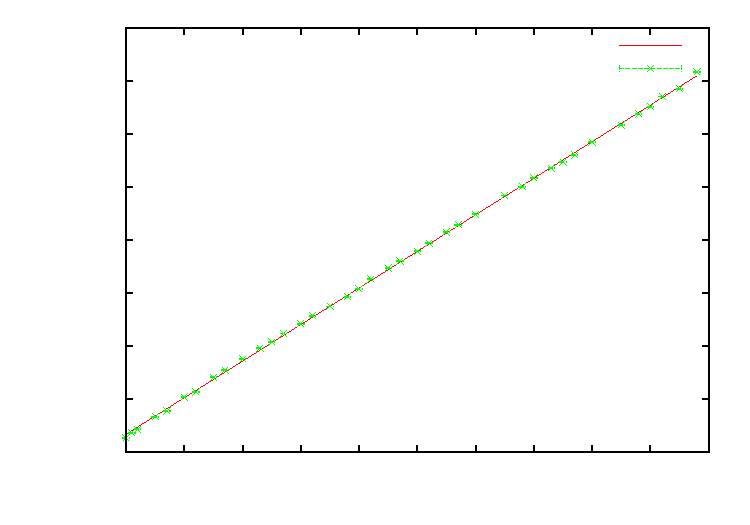
\includegraphics{gas1p}}%
    \gplfronttext
  \end{picture}%
\endgroup

\caption{Der Druck ist in der Abbildung als Funktion für die Erwärmung aufgetragen. Mit Fehlerbalken von $\pm$0.08 (Annahmemessfehler) und einer linearen Regression durch die Messpunkte}
\label{fig:gas1}
\end{figure}

Aus der Graphik \ref{fig:gas1} ergeben sich die hier aufgeführten Werte.
\begin{align*}
	\text{m} &= (312.1\pm 2)\si{\pascal/\celsius}\\
	\text{b} &= (101173\pm112)\si{\pascal}\\
\end{align*}
Die Geradengleichung $y=mx+b$ wird nun nach x umgestellt. Es ergibt sich $x=y-b/m$

Zu berechnen ist nun die Temperatur bei einem Druck von p=0. Diese Temperatur wird aus als Nullpunktstemperatur bezeichnet, da nichts kälter werden kann. Dazu berechnen wir einfach den x-Achsenabschnitt und setzten dafür y=0.

$$\text{T}=(-308.5\pm2.1)\si{\celsius}$$


Unter der Annahme eines idealen Gases ergibt sich folgende Fehlerfortpflanzung.
\begin{align}
	\sigma_{x}=\sqrt{\sigma_\text{b}^2\left(\frac{-1}{\text{m}}\right)^2+\sigma_\text{m}^2\left(\frac{\text{b}}{\text{m}^2}\right)^2}\label{eq:fegas}
\end{align}


\subsubsection{Abkühlung des Gases}
\label{sec:gas2}
Da sich bei den Messgeräten zur Abkühlung des Gases nichts verändert hat, werden hier auch weider die Messwerte mit 2 multipliziert und der Normaldruck (1013hPa) hinzu addiert.In der Graphik \ref{fig:gas2} aufgetragen ist der Druck p gegen die jeweilige Temperatur.
\begin{figure}[!h]
\centering
% GNUPLOT: LaTeX picture with Postscript
\begingroup
  \makeatletter
  \providecommand\color[2][]{%
    \GenericError{(gnuplot) \space\space\space\@spaces}{%
      Package color not loaded in conjunction with
      terminal option `colourtext'%
    }{See the gnuplot documentation for explanation.%
    }{Either use 'blacktext' in gnuplot or load the package
      color.sty in LaTeX.}%
    \renewcommand\color[2][]{}%
  }%
  \providecommand\includegraphics[2][]{%
    \GenericError{(gnuplot) \space\space\space\@spaces}{%
      Package graphicx or graphics not loaded%
    }{See the gnuplot documentation for explanation.%
    }{The gnuplot epslatex terminal needs graphicx.sty or graphics.sty.}%
    \renewcommand\includegraphics[2][]{}%
  }%
  \providecommand\rotatebox[2]{#2}%
  \@ifundefined{ifGPcolor}{%
    \newif\ifGPcolor
    \GPcolortrue
  }{}%
  \@ifundefined{ifGPblacktext}{%
    \newif\ifGPblacktext
    \GPblacktexttrue
  }{}%
  % define a \g@addto@macro without @ in the name:
  \let\gplgaddtomacro\g@addto@macro
  % define empty templates for all commands taking text:
  \gdef\gplbacktext{}%
  \gdef\gplfronttext{}%
  \makeatother
  \ifGPblacktext
    % no textcolor at all
    \def\colorrgb#1{}%
    \def\colorgray#1{}%
  \else
    % gray or color?
    \ifGPcolor
      \def\colorrgb#1{\color[rgb]{#1}}%
      \def\colorgray#1{\color[gray]{#1}}%
      \expandafter\def\csname LTw\endcsname{\color{white}}%
      \expandafter\def\csname LTb\endcsname{\color{black}}%
      \expandafter\def\csname LTa\endcsname{\color{black}}%
      \expandafter\def\csname LT0\endcsname{\color[rgb]{1,0,0}}%
      \expandafter\def\csname LT1\endcsname{\color[rgb]{0,1,0}}%
      \expandafter\def\csname LT2\endcsname{\color[rgb]{0,0,1}}%
      \expandafter\def\csname LT3\endcsname{\color[rgb]{1,0,1}}%
      \expandafter\def\csname LT4\endcsname{\color[rgb]{0,1,1}}%
      \expandafter\def\csname LT5\endcsname{\color[rgb]{1,1,0}}%
      \expandafter\def\csname LT6\endcsname{\color[rgb]{0,0,0}}%
      \expandafter\def\csname LT7\endcsname{\color[rgb]{1,0.3,0}}%
      \expandafter\def\csname LT8\endcsname{\color[rgb]{0.5,0.5,0.5}}%
    \else
      % gray
      \def\colorrgb#1{\color{black}}%
      \def\colorgray#1{\color[gray]{#1}}%
      \expandafter\def\csname LTw\endcsname{\color{white}}%
      \expandafter\def\csname LTb\endcsname{\color{black}}%
      \expandafter\def\csname LTa\endcsname{\color{black}}%
      \expandafter\def\csname LT0\endcsname{\color{black}}%
      \expandafter\def\csname LT1\endcsname{\color{black}}%
      \expandafter\def\csname LT2\endcsname{\color{black}}%
      \expandafter\def\csname LT3\endcsname{\color{black}}%
      \expandafter\def\csname LT4\endcsname{\color{black}}%
      \expandafter\def\csname LT5\endcsname{\color{black}}%
      \expandafter\def\csname LT6\endcsname{\color{black}}%
      \expandafter\def\csname LT7\endcsname{\color{black}}%
      \expandafter\def\csname LT8\endcsname{\color{black}}%
    \fi
  \fi
  \setlength{\unitlength}{0.0500bp}%
  \begin{picture}(7200.00,5040.00)%
    \gplgaddtomacro\gplbacktext{%
      \csname LTb\endcsname%
      \put(1386,704){\makebox(0,0)[r]{\strut{} 1000}}%
      \put(1386,1286){\makebox(0,0)[r]{\strut{} 1050}}%
      \put(1386,1867){\makebox(0,0)[r]{\strut{} 1100}}%
      \put(1386,2449){\makebox(0,0)[r]{\strut{} 1150}}%
      \put(1386,3031){\makebox(0,0)[r]{\strut{} 1200}}%
      \put(1386,3613){\makebox(0,0)[r]{\strut{} 1250}}%
      \put(1386,4194){\makebox(0,0)[r]{\strut{} 1300}}%
      \put(1386,4776){\makebox(0,0)[r]{\strut{} 1350}}%
      \put(1518,484){\makebox(0,0){\strut{} 0}}%
      \put(2062,484){\makebox(0,0){\strut{} 10}}%
      \put(2606,484){\makebox(0,0){\strut{} 20}}%
      \put(3150,484){\makebox(0,0){\strut{} 30}}%
      \put(3694,484){\makebox(0,0){\strut{} 40}}%
      \put(4238,484){\makebox(0,0){\strut{} 50}}%
      \put(4782,484){\makebox(0,0){\strut{} 60}}%
      \put(5326,484){\makebox(0,0){\strut{} 70}}%
      \put(5870,484){\makebox(0,0){\strut{} 80}}%
      \put(6414,484){\makebox(0,0){\strut{} 90}}%
      \put(6958,484){\makebox(0,0){\strut{} 100}}%
      \put(484,2740){\rotatebox{90}{\makebox(0,0){\strut{}Druck [hPa]}}}%
      \put(4238,154){\makebox(0,0){\strut{}Temperatur [$\si{\celsius}$]}}%
    }%
    \gplgaddtomacro\gplfronttext{%
      \csname LTb\endcsname%
      \put(5971,4603){\makebox(0,0)[r]{\strut{}Messwerte}}%
      \csname LTb\endcsname%
      \put(5971,4383){\makebox(0,0)[r]{\strut{}lineare Regression}}%
    }%
    \gplbacktext
    \put(0,0){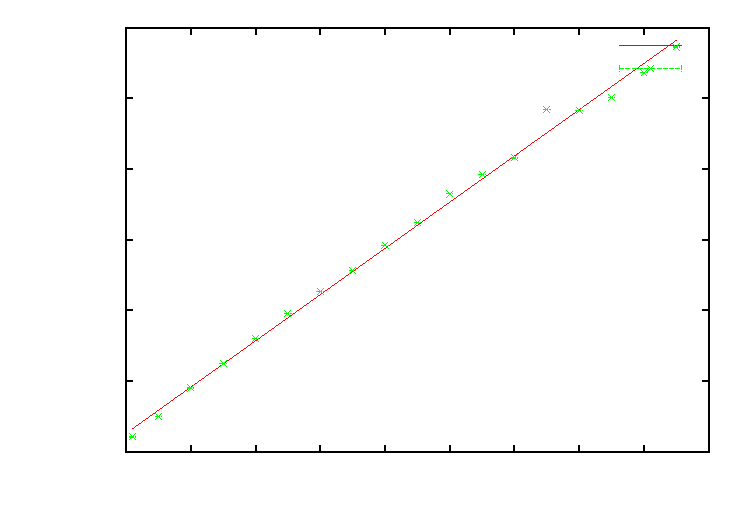
\includegraphics{gas2p}}%
    \gplfronttext
  \end{picture}%
\endgroup

\caption{lineare Regression der Temperatur gegen den Druck für die Abkühlung}
\label{fig:gas2}
\end{figure}
Wie bei der Erwärmung ist die Rechnung für die Nullpunktstemperatur die gleiche. Die Fehlerfortpflanzungsformel ist weiterhin:
\begin{align}
	\sigma_{x}=\sqrt{\sigma_\text{b}^2\left(\frac{-1}{\text{m}}\right)^2+\sigma_\text{m}^2\left(\frac{\text{b}}{\text{m}^2}\right)^2}\label{eq:fegas}
\end{align}


Aus der linearen Regression der Graphik, ergeben sich folgende Werte.
\begin{align}
	\text{m} &= (327\pm5)\si{\pascal/\celsius}\\
	\text{b} &= (101296\pm260)\si{\pascal}
\end{align}
Setzt man wieder y=0, so ergibt sich aus der Formel \eqref{eq:gasfor} der folgende Nullpunktstemperaturwert.
$$\text{T}=(-322.8\pm5.2)\si{\celsius}$$

\subsubsection{gewichteter Mittelwert}
Der gewichtet Mittelwert von der Erwärmung und der Abkühlung des Gases ist:
$$\shadowbox{$\overline{\text{T}}=(-310.1\pm1.9)\si{\celsius}$}$$
Der  Literaturwert von T=$-273.15\si{\celsius}$ an hat somit zu unserem  Wert eine Abweichung von 8.8\%.

\subsection{Spezifische Wärme von Luft}
\subsubsection{Freiheitsgrade der Luft}
Für den zweiten Teil und der Errechnung der Molwärme $c_V$ von Luft muss zunächst aus den gemessenen Daten die Druckänderung jeder Entladung ausgerechnet werden. Mit der Formel $\Delta p=\varrho_{H_2O}gh(1+r_1^2 / r_2^2 )$, lässt sich die Höhe der Wassersäule ausrechnen.Die Werte für $r_1$= 2.0 mm und $r_2$=9.2mm sind in der Praktikumsanleitung[S.73] zu finden.$\Delta Q$, also die Änderung der Energie lässt sich mit der Formel aus der Theorie berechnen. Die Kapazität berechnet sich aus zwei parallel geschalteten Kondensatoren mit jeweils 10$\mu$F.
Mit der Gauß'schen Fehlerpfortpflanzung ergibt sich für $\Delta Q$ ein Fehler von:
$$\sigma_{\Delta Q}=\sigma_U \cdot CU$$
Der Fehler für $\Delta p$ ist:
$$\sigma_{\Delta p}=\sigma_h \varrho g \left(1+r_1^2/r_2^2 \right)$$

Die Graphik \ref{fig:druckwarm} zeigt die Druckänderung von Luft gegen die Kondensatorenergie aufgetragen.
\begin{figure}[!h]
\centering
% GNUPLOT: LaTeX picture with Postscript
\begingroup
  \makeatletter
  \providecommand\color[2][]{%
    \GenericError{(gnuplot) \space\space\space\@spaces}{%
      Package color not loaded in conjunction with
      terminal option `colourtext'%
    }{See the gnuplot documentation for explanation.%
    }{Either use 'blacktext' in gnuplot or load the package
      color.sty in LaTeX.}%
    \renewcommand\color[2][]{}%
  }%
  \providecommand\includegraphics[2][]{%
    \GenericError{(gnuplot) \space\space\space\@spaces}{%
      Package graphicx or graphics not loaded%
    }{See the gnuplot documentation for explanation.%
    }{The gnuplot epslatex terminal needs graphicx.sty or graphics.sty.}%
    \renewcommand\includegraphics[2][]{}%
  }%
  \providecommand\rotatebox[2]{#2}%
  \@ifundefined{ifGPcolor}{%
    \newif\ifGPcolor
    \GPcolortrue
  }{}%
  \@ifundefined{ifGPblacktext}{%
    \newif\ifGPblacktext
    \GPblacktexttrue
  }{}%
  % define a \g@addto@macro without @ in the name:
  \let\gplgaddtomacro\g@addto@macro
  % define empty templates for all commands taking text:
  \gdef\gplbacktext{}%
  \gdef\gplfronttext{}%
  \makeatother
  \ifGPblacktext
    % no textcolor at all
    \def\colorrgb#1{}%
    \def\colorgray#1{}%
  \else
    % gray or color?
    \ifGPcolor
      \def\colorrgb#1{\color[rgb]{#1}}%
      \def\colorgray#1{\color[gray]{#1}}%
      \expandafter\def\csname LTw\endcsname{\color{white}}%
      \expandafter\def\csname LTb\endcsname{\color{black}}%
      \expandafter\def\csname LTa\endcsname{\color{black}}%
      \expandafter\def\csname LT0\endcsname{\color[rgb]{1,0,0}}%
      \expandafter\def\csname LT1\endcsname{\color[rgb]{0,1,0}}%
      \expandafter\def\csname LT2\endcsname{\color[rgb]{0,0,1}}%
      \expandafter\def\csname LT3\endcsname{\color[rgb]{1,0,1}}%
      \expandafter\def\csname LT4\endcsname{\color[rgb]{0,1,1}}%
      \expandafter\def\csname LT5\endcsname{\color[rgb]{1,1,0}}%
      \expandafter\def\csname LT6\endcsname{\color[rgb]{0,0,0}}%
      \expandafter\def\csname LT7\endcsname{\color[rgb]{1,0.3,0}}%
      \expandafter\def\csname LT8\endcsname{\color[rgb]{0.5,0.5,0.5}}%
    \else
      % gray
      \def\colorrgb#1{\color{black}}%
      \def\colorgray#1{\color[gray]{#1}}%
      \expandafter\def\csname LTw\endcsname{\color{white}}%
      \expandafter\def\csname LTb\endcsname{\color{black}}%
      \expandafter\def\csname LTa\endcsname{\color{black}}%
      \expandafter\def\csname LT0\endcsname{\color{black}}%
      \expandafter\def\csname LT1\endcsname{\color{black}}%
      \expandafter\def\csname LT2\endcsname{\color{black}}%
      \expandafter\def\csname LT3\endcsname{\color{black}}%
      \expandafter\def\csname LT4\endcsname{\color{black}}%
      \expandafter\def\csname LT5\endcsname{\color{black}}%
      \expandafter\def\csname LT6\endcsname{\color{black}}%
      \expandafter\def\csname LT7\endcsname{\color{black}}%
      \expandafter\def\csname LT8\endcsname{\color{black}}%
    \fi
  \fi
  \setlength{\unitlength}{0.0500bp}%
  \begin{picture}(7200.00,5040.00)%
    \gplgaddtomacro\gplbacktext{%
      \csname LTb\endcsname%
      \put(1254,704){\makebox(0,0)[r]{\strut{} 0}}%
      \put(1254,1383){\makebox(0,0)[r]{\strut{} 50}}%
      \put(1254,2061){\makebox(0,0)[r]{\strut{} 100}}%
      \put(1254,2740){\makebox(0,0)[r]{\strut{} 150}}%
      \put(1254,3419){\makebox(0,0)[r]{\strut{} 200}}%
      \put(1254,4097){\makebox(0,0)[r]{\strut{} 250}}%
      \put(1254,4776){\makebox(0,0)[r]{\strut{} 300}}%
      \put(1386,484){\makebox(0,0){\strut{} 0}}%
      \put(2315,484){\makebox(0,0){\strut{} 0.5}}%
      \put(3243,484){\makebox(0,0){\strut{} 1}}%
      \put(4172,484){\makebox(0,0){\strut{} 1.5}}%
      \put(5101,484){\makebox(0,0){\strut{} 2}}%
      \put(6029,484){\makebox(0,0){\strut{} 2.5}}%
      \put(6958,484){\makebox(0,0){\strut{} 3}}%
      \put(484,2740){\rotatebox{90}{\makebox(0,0){\strut{}$\Delta p$ [Pa]}}}%
      \put(4172,154){\makebox(0,0){\strut{}$\Delta Q$ [J]}}%
    }%
    \gplgaddtomacro\gplfronttext{%
      \csname LTb\endcsname%
      \put(3894,4603){\makebox(0,0)[r]{\strut{}Messwerte}}%
      \csname LTb\endcsname%
      \put(3894,4383){\makebox(0,0)[r]{\strut{}Lineare Regression}}%
    }%
    \gplbacktext
    \put(0,0){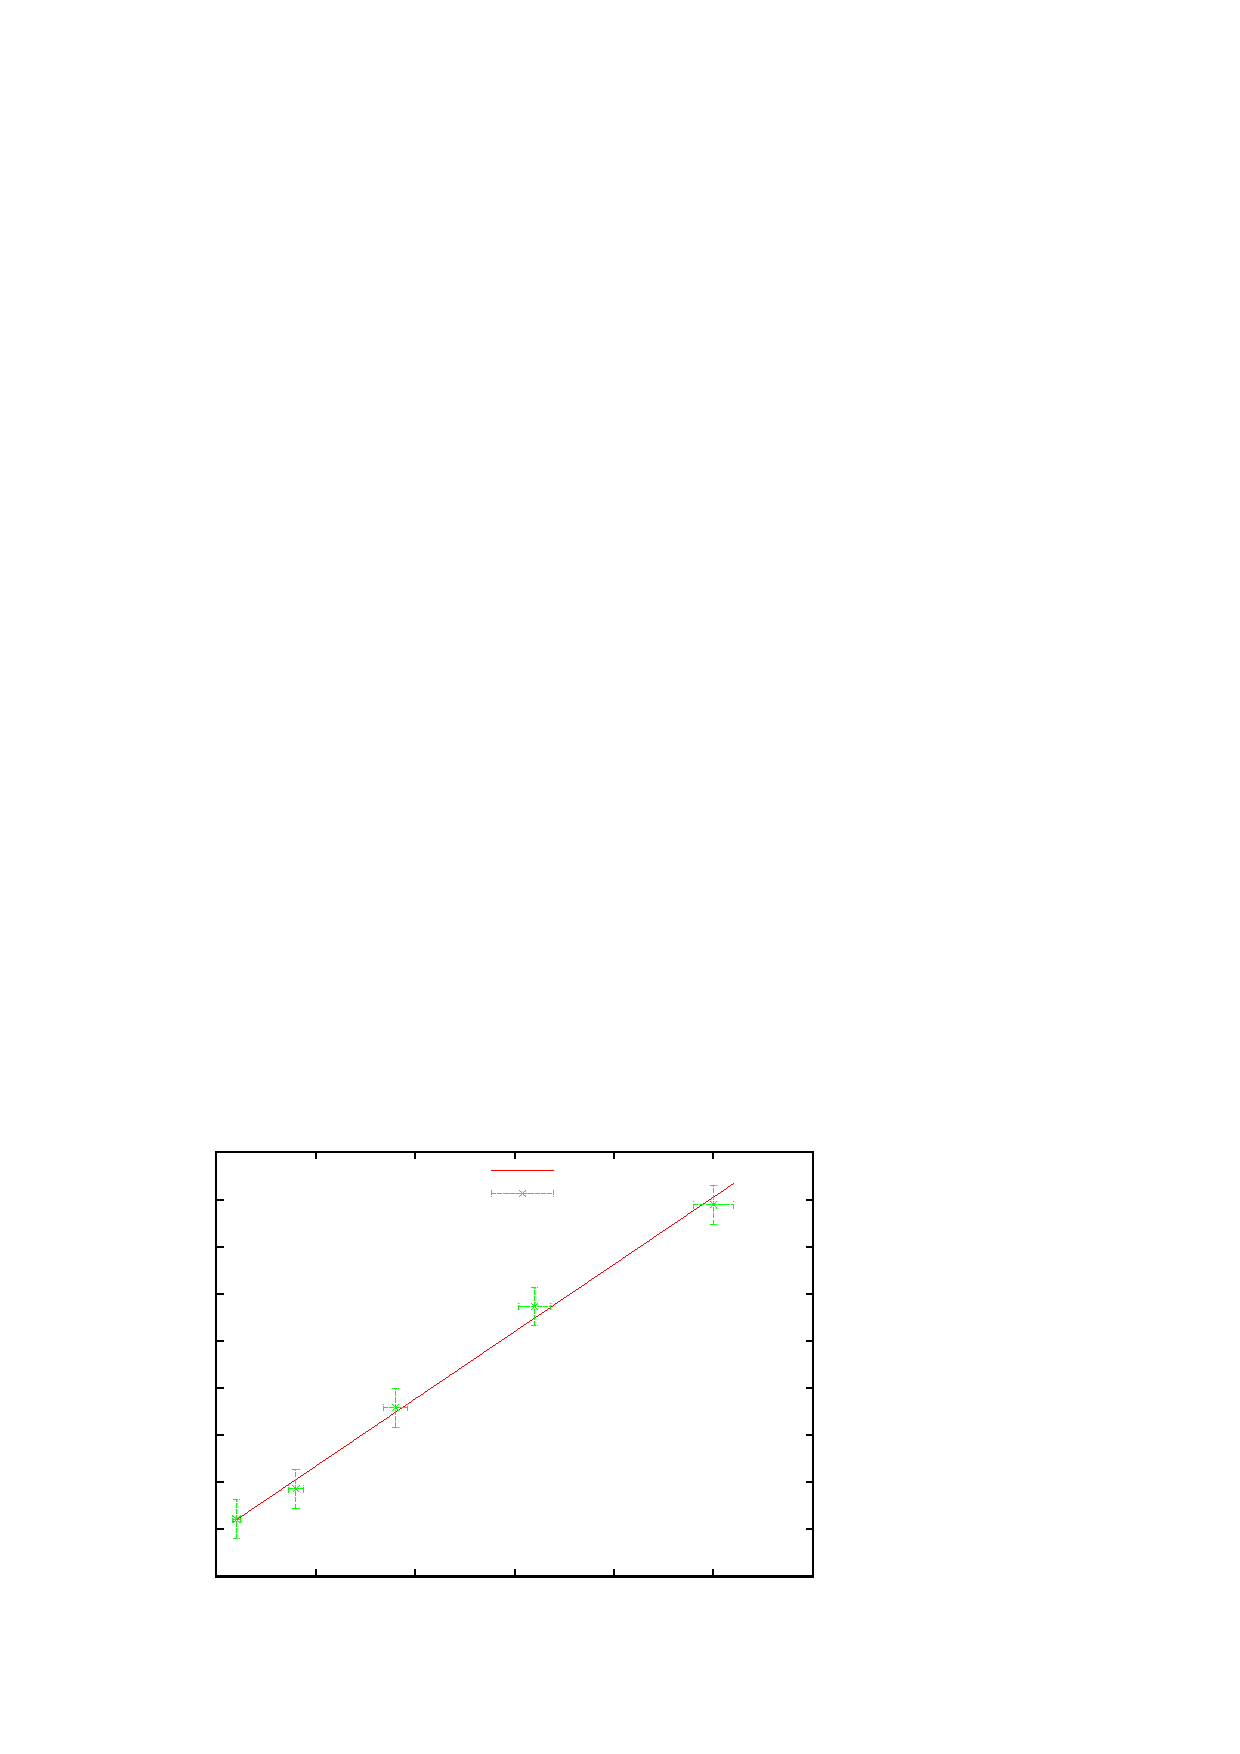
\includegraphics{kondwarm}}%
    \gplfronttext
  \end{picture}%
\endgroup

\caption{Energie des Kondensators aufgetragen gegen die Änderung im Druck}
\label{fig:druckwarm}
\end{figure}
Mit der Steigung,
 $m=(142.7\pm5.5)\frac{\text{J}}{\text{Pa}}$ lässt sich über die Formel aus der Theorie  die Freiheitsgrade des Gases bestimmen.
.

Es wird angenommen, dass $\Delta V=0$ ist, da das Volumen konstant bleibt.
Setzt man $\frac{\Delta Q}{\Delta p}=\frac1m$ gilt:
\begin{align}
	f/2= \frac{ \Delta Q}{V\cdot \Delta p}=\frac{1}{V\cdot m}
\end{align}

Die gegebenen Maße für das Volumen des Zylinders sind r=0.044$\pm$0.002m und eine Höhe h=0.4$\pm$0.005



Es ergibt sich mit der Gauß'schen Fehlerfortpflanzung .
\begin{align}
	\sigma_f=\sqrt{\sigma_V^2\left(\frac{-2}{V^2\cdot m}\right)^2+\sigma_m^2\left(\frac{-2}{V\cdot m^2}\right)^2}
\end{align}

Es ergibt sich für Luft folgende Freiheitsgrade:
$$\shadowbox{$f=(6.4\pm1.8 )$}$$

Dies entspricht eine Abweichung von 21.9\% zu den angenommenen 5 Freiheitsgraden die Luft in idealisierter Form hat.

\subsubsection{Spezifische Wärme $c_v$}
Mit den Freiheitsgraden lässt sich die Spezifische Wärme $c_v$ der Luft berechnen.
Dafür nutzt man die Formel:
\begin{align}
	c_v=\frac{f\cdot R}{2}
\end{align}
Die ist mit einem Fortpflanzungsfehler  für f behaftet. 
\begin{align}
	\sigma_{c_v}= \sqrt{\sigma_f^2\left(\frac{R}{2}\right)^2}
\end{align}
Es ergibt sich ein Wert für die spezifische Wärme von Luft.
$$c_v=(26.6\pm7.5)\si{\joule/\mol\kelvin}$$
Der Literaturwert ist $c_v=20.7\si{\joule/\mol\kelvin}$ [Gerthsen- Seite 260].

\section{Diskussion}
\label{sec:diskussion}
\subsection{Gasthermometer}
Die Abweichung des gewichteten Mittelwertes der beiden Messungen zu dem Literaturwert, beträgt 8.8\%. Der Literaturwert liegt nicht im Fehlerintervall des aus dem experimentell bestimmten Wert.
Dies könnte verschiedene Ursachen haben: Wir gehen davon aus, dass eine der möglichen Fehlerquellen das nicht vollständige Eintauchen des Glasbehälters in das Eiswasser sein könnte. Das Thermometer sehen wir auch als mögliche Fehlerquelle an, da es im Vergleich zu dem Druckmessgerät ziemlich schwer abzulesen war. Trotzdem ist eine Abweichung von ca. 9 \% aus unserer Ansicht nicht zu groß, eher hätten wir größere Annahmefehler abschätzen sollen. 


\subsection{Spezifische Wärme der Luft}
Die Abweichung unseres Wertes zum Literaturwert beträgt 22.1\% dieser Wert ist zwar recht groß, jedoch liegt der Literaturwert in dem Fehlerintervall woher wir davon ausgehen können, dass die Annahmefehler gut abgeschätzt wurden. Eine Abweichung von 22.1\% ist wohl durch den Versuch an sich zu begründen, da es nur sehr schwer war die Höhe der Wassersäule  abzulesen. Hier ist es offensichtlichzu größeren Ablesefehler gekommen.
\bibliography{literatur}
\bibliographystyle{babalpha}
\end{document}
